\documentclass[11pt,utf8,notheorems,compress,t]{beamer}
\usepackage{etex}
\usepackage{xspace}
\usepackage{wrapfig}

\usepackage{pgfpages}
%\setbeameroption{show notes on second screen}
\setbeamertemplate{note page}[plain]
\newcommand{\jnote}[2]{\only<#1>{\note{\setlength\parskip{\medskipamount}\justifying\footnotesize#2\par}}}
%\newcommand{\jnote}[2]{}

% Workaround for the issue described at
% https://tex.stackexchange.com/questions/164406/beamer-using-href-in-notes.
\newcommand{\fixedhref}[2]{\makebox[0pt][l]{\hspace*{\paperwidth}\href{#1}{#2}}\href{#1}{#2}}

\usepackage[english]{babel}

\usepackage{graphbox}
\usepackage{mathtools}
\usepackage{booktabs}
\usepackage{stmaryrd}
\usepackage{array}
\usepackage{ragged2e}
\usepackage{multicol}
\usepackage{tabto}
\usepackage{xstring}
\usepackage{ifthen}
\usepackage[normalem]{ulem}
\usepackage[all]{xy}
\xyoption{rotate}
\usepackage{tikz}
\usetikzlibrary{calc,shapes,shapes.callouts,shapes.arrows,patterns,fit,backgrounds,decorations.pathmorphing,positioning}
\hypersetup{colorlinks=true}

\usepackage{pifont}
\newcommand{\cmark}{\ding{51}}
\newcommand{\xmark}{\ding{55}}
\DeclareSymbolFont{extraup}{U}{zavm}{m}{n}
\DeclareMathSymbol{\varheart}{\mathalpha}{extraup}{86}

\graphicspath{{images/}}

\usepackage[protrusion=true,expansion=true]{microtype}

\setlength\parskip{\medskipamount}
\setlength\parindent{0pt}

\title{Embracing the generic prime ideal: the tale of an enchanting mathematical phantom}
\author{Ingo Blechschmidt}
\date{March 11th, 2022}

\useinnertheme{rectangles}
\setbeamerfont{block title}{size={}}

\useinnertheme{rectangles}

\usecolortheme{orchid}
\usecolortheme{seahorse}
\definecolor{mypurple}{RGB}{150,0,255}
\setbeamercolor{structure}{fg=mypurple}
\definecolor{myred}{RGB}{150,0,0}
\setbeamercolor*{title}{bg=mypurple,fg=white}
\setbeamercolor*{titlelike}{bg=mypurple,fg=white}
\setbeamercolor{frame}{bg=black}

\usefonttheme{serif}
\usepackage[T1]{fontenc}
\usepackage{libertine}

% lifted from https://arxiv.org/abs/1506.08870
\DeclareFontFamily{U}{min}{}
\DeclareFontShape{U}{min}{m}{n}{<-> udmj30}{}
\newcommand\yon{\!\text{\usefont{U}{min}{m}{n}\symbol{'210}}\!}

\newcommand{\A}{\mathcal{A}}
\newcommand{\B}{\mathcal{B}}
\newcommand{\C}{\mathcal{C}}
\newcommand{\M}{\mathcal{M}}
\renewcommand{\AA}{\mathbb{A}}
\newcommand{\E}{\mathcal{E}}
\newcommand{\F}{\mathcal{F}}
\newcommand{\G}{\mathcal{G}}
\newcommand{\J}{\mathcal{J}}
\newcommand{\GG}{\mathbb{G}}
\renewcommand{\O}{\mathcal{O}}
\newcommand{\K}{\mathcal{K}}
\newcommand{\NN}{\mathbb{N}}
\newcommand{\QQ}{\mathbb{Q}}
\newcommand{\RR}{\mathbb{R}}
\newcommand{\TT}{\mathbb{T}}
\newcommand{\PP}{\mathbb{P}}
\newcommand{\ZZ}{\mathbb{Z}}
\newcommand{\CC}{\mathbb{C}}
\renewcommand{\P}{\mathcal{P}}
\newcommand{\aaa}{\mathfrak{a}}
\newcommand{\ppp}{\mathfrak{p}}
\newcommand{\fff}{\mathfrak{f}}
\newcommand{\defeq}{\vcentcolon=}
\newcommand{\defeqv}{\vcentcolon\equiv}
\newcommand{\Sh}{\mathrm{Sh}}
\newcommand{\GL}{\mathrm{GL}}
\newcommand{\Zar}{\mathrm{Zar}}
\newcommand{\op}{\mathrm{op}}
\newcommand{\Set}{\mathrm{Set}}
\newcommand{\Eff}{\mathrm{Ef{}f}}
\newcommand{\Sch}{\mathrm{Sch}}
\newcommand{\Aff}{\mathrm{Aff}}
\newcommand{\Ring}{\mathrm{Ring}}
\newcommand{\LocRing}{\mathrm{LocRing}}
\newcommand{\LRS}{\mathrm{LRS}}
\newcommand{\Hom}{\mathrm{Hom}}
\newcommand{\Spec}{\mathrm{Spec}}
\newcommand{\lra}{\longrightarrow}
\newcommand{\RelSpec}{\operatorname{Spec}}
\renewcommand{\_}{\mathpunct{.}}
\newcommand{\?}{\,{:}\,}
\newcommand{\ul}[1]{\underline{#1}}
\newcommand{\affl}{\ensuremath{{\ul{\ensuremath{\AA}}^1}}}
\newcommand{\Ll}{\text{iff}}
\newcommand{\inv}{inv.\@}
\newcommand{\seq}[1]{\mathrel{\vdash\!\!\!_{#1}}}
\newcommand{\hg}{\mathbin{:}}  % homogeneous coordinates
\newcommand{\brak}[1]{{\llbracket{#1}\rrbracket}}
\newcommand{\pt}{\mathrm{pt}}
\newcommand{\Loc}{\mathrm{Loc}}
\newcommand{\Top}{\mathrm{Top}}
\newcommand{\effective}{ef{}fective\xspace}

%\setbeamertemplate{blocks}[rectangles][shadow=false]

\newenvironment{indentblock}{%
  \list{}{\leftmargin\leftmargin}%
  \item\relax
}{%
  \endlist
}

% Adapted from https://latex.org/forum/viewtopic.php?t=2251 (Stefan Kottwitz)
\newenvironment<>{hilblock}{
  \begin{center}
    \begin{minipage}{9.05cm}
      \setlength{\textwidth}{9.05cm}
      \begin{actionenv}#1
        \def\insertblocktitle{}
        \par
        \usebeamertemplate{block begin}}{
        \par
        \usebeamertemplate{block end}
      \end{actionenv}
    \end{minipage}
  \end{center}}

\newcommand{\bignumber}[1]{
  \renewcommand{\insertenumlabel}{#1}\scalebox{1.5}{\usebeamertemplate{enumerate item}}
}
\newcommand{\normalnumber}[1]{
  \renewcommand{\insertenumlabel}{#1}\scalebox{1.0}{\usebeamertemplate{enumerate item}}
}
\newcommand{\bigheart}{
\includegraphics{heart}}

\newenvironment{changemargin}[2]{%
  \begin{list}{}{%
    \setlength{\topsep}{0pt}%
    \setlength{\leftmargin}{#1}%
    \setlength{\rightmargin}{#2}%
    \setlength{\listparindent}{\parindent}%
    \setlength{\itemindent}{\parindent}%
    \setlength{\parsep}{\parskip}%
  }%
  \item[]}{\end{list}}

\tikzset{
  invisible/.style={opacity=0,text opacity=0},
  visible on/.style={alt={#1{}{invisible}}},
  alt/.code args={<#1>#2#3}{%
    \alt<#1>{\pgfkeysalso{#2}}{\pgfkeysalso{#3}}}
}

\newcommand{\pointthis}[3]{%
  \tikz[remember picture,baseline]{
    \node[anchor=base,inner sep=0,outer sep=0] (#2) {#2};
    \node[visible on=#1,overlay,rectangle callout,callout relative pointer={(0.3cm,0.5cm)},fill=blue!20] at ($(#2.north)+(-0.1cm,-1.1cm)$) {#3};
  }%
}

\tikzset{
  invisible/.style={opacity=0,text opacity=0},
  visible on/.style={alt={#1{}{invisible}}},
  alt/.code args={<#1>#2#3}{%
    \alt<#1>{\pgfkeysalso{#2}}{\pgfkeysalso{#3}}}
}

\newcommand{\hcancel}[5]{%
  \tikz[baseline=(tocancel.base)]{
    \node[inner sep=0pt,outer sep=0pt] (tocancel) {#1};
    \draw[red!80, line width=0.4mm] ($(tocancel.south west)+(#2,#3)$) -- ($(tocancel.north east)+(#4,#5)$);
  }%
}

\newcommand{\explain}[7]{%
  \tikz[remember picture,baseline]{
    \node[anchor=base,inner sep=2pt,outer sep=0,fill=#3,rounded corners] (label) {#1};
    \node[anchor=north,visible on=<#2>,overlay,rectangle callout,rounded corners,callout
    relative pointer={(0.0cm,0.5cm)+(0.0cm,#6)},fill=#3] at ($(label.south)+(0,-0.3cm)+(#4,#5)$) {#7};
  }%
}

\newcommand{\explainstub}[2]{%
  \tikz[remember picture,baseline]{
    \node[anchor=base,inner sep=2pt,outer sep=0,fill=#2,rounded corners] (label) {#1};
  }%
}

\newcommand{\squiggly}[1]{%
  \tikz[remember picture,baseline]{
    \node[anchor=base,inner sep=0,outer sep=0] (label) {#1};
    \draw[thick,color=red!80,decoration={snake,amplitude=0.5pt,segment
    length=3pt},decorate] ($(label.south west) + (0,-2pt)$) -- ($(label.south east) + (0,-2pt)$);
  }%
}

\setbeamertemplate{frametitle}[default][center]

% Adapted from https://latex.org/forum/viewtopic.php?t=2251 (Stefan Kottwitz)
\newenvironment<>{varblock}[2]{\begin{varblockextra}{#1}{#2}{}}{\end{varblockextra}}
\newenvironment<>{varblockextra}[3]{
  %\begin{center}
    \begin{minipage}{#1}
      \begin{actionenv}#4
	\def\insertblocktitle{\vspace*{-1em}}
        \def\varblockextraend{#3}
	\usebeamertemplate{block begin}}{
        \par
        \usebeamertemplate{block end}
        \varblockextraend
      \end{actionenv}
    \end{minipage}
  }
  %\end{center}}


\setbeamertemplate{navigation symbols}{}

\newcounter{framenumberpreappendix}
\newcommand{\backupstart}{
  \setcounter{framenumberpreappendix}{\value{framenumber}}
}
\newcommand{\backupend}{
  \addtocounter{framenumberpreappendix}{-\value{framenumber}}
  \addtocounter{framenumber}{\value{framenumberpreappendix}}
}

\newcommand{\insertframeextra}{}
\setbeamertemplate{footline}{%
  \begin{beamercolorbox}[wd=\paperwidth,ht=2.25ex,dp=1ex,right,rightskip=1mm,leftskip=1mm]{}%
    % \inserttitle
    \hfill
    \insertframenumber\insertframeextra\,/\,\inserttotalframenumber
  \end{beamercolorbox}%
  \vskip0pt%
}


\newcommand{\hil}[1]{{\usebeamercolor[fg]{item}{\textbf{#1}}}}
\newcommand{\bad}[1]{\textcolor{red!90}{\textnormal{#1}}}

\newcommand{\subhead}[1]{{\centering\textcolor{gray}{\hrulefill}\quad\textnormal{\hil{#1}}\quad\textcolor{gray}{\hrulefill}\par\vspace*{-0.6em}}}

\newcommand{\speak}[2]{\textcolor{blue!80}{$#1 \models #2$}}
\newcommand{\simplespeak}[1]{\textcolor{blue!80}{`#1'}}

\newcommand{\triang}{\hil{$\blacktriangleright$}\xspace}

\setbeamertemplate{itemize item}{$\blacktriangleright$}

\begin{document}

\addtocounter{framenumber}{-1}

%{\usebackgroundtemplate{\begin{minipage}{\paperwidth}\vspace*{4.95cm}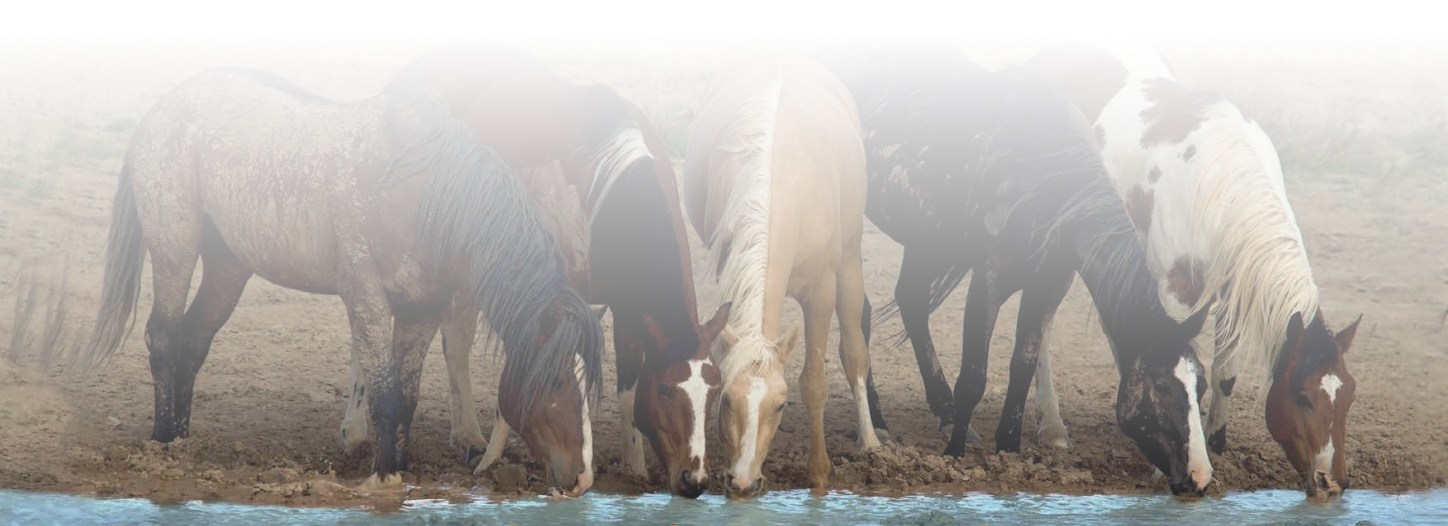
\includegraphics[width=\paperwidth]{topos-horses}\end{minipage}}
{
\begin{frame}[c]
  \centering

  \bigskip
  \bigskip
  
\includegraphics[width=0.4\textwidth]{phantoms}
  \bigskip
  \bigskip
  \bigskip

  Embracing the generic prime ideal: \\
  \hil{the tale of an enchanting mathematical phantom}

  \scriptsize
  \textit{-- an invitation --}
  \bigskip
  \bigskip
  \bigskip

  \textit{Antwerp Algebra Colloquium} \\
  \color{black}
  March 11th, 2022

  \bigskip
  \bigskip

  \color{black}
  Ingo Blechschmidt \\
  University of Augsburg
  \bigskip
  \bigskip
  \bigskip

  \par
\end{frame}}

\begin{frame}[t]{Mathematical phantoms}
  \begin{columns}[T]
    \begin{column}{0.3\textwidth}
      \centering
      
\includegraphics[width=\textwidth]{wraith-portrait} \\
      \scriptsize
      Gavin Wraith
    \end{column}

    \begin{column}{0.7\textwidth}
      \emph{One of the recurring themes of mathematics, \\
      and one that I have always found seductive, \\
      is that of \\\medskip
      \triang the nonexistent entity which ought to be there \\
      \phantom{\triang}but apparently is not; \\\medskip
      \triang which nevertheless obtrudes its effects so \\
      \phantom{\triang}convincingly that
      one is forced to concede \\
      \phantom{\triang}a broader notion of existence.}
    \end{column}
  \end{columns}

  \bigskip
  \subhead{Examples}
  \bigskip

  \mbox{\begin{minipage}{0.15\textwidth}
    \centering\small
    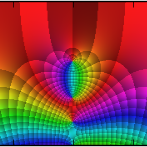
\includegraphics[height=5em]{zeta-function} \\
    $\mathbb{C}$
  \end{minipage}\quad
  \begin{minipage}{0.20\textwidth}
    \centering\small
    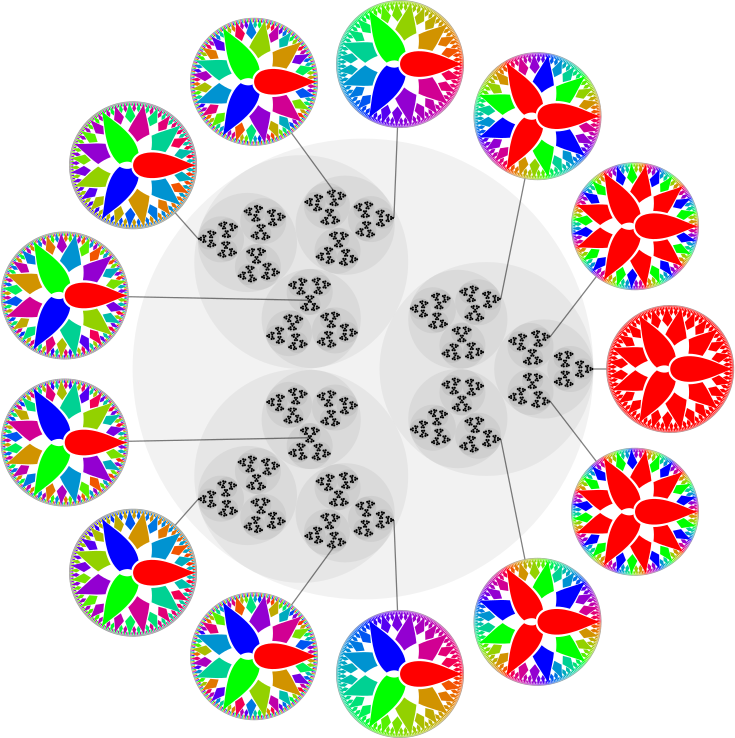
\includegraphics[height=5em]{3-adic-numbers} \\
    $\mathbb{Q}_p$
  \end{minipage}\quad
  \begin{minipage}{0.20\textwidth}
    \centering\small
    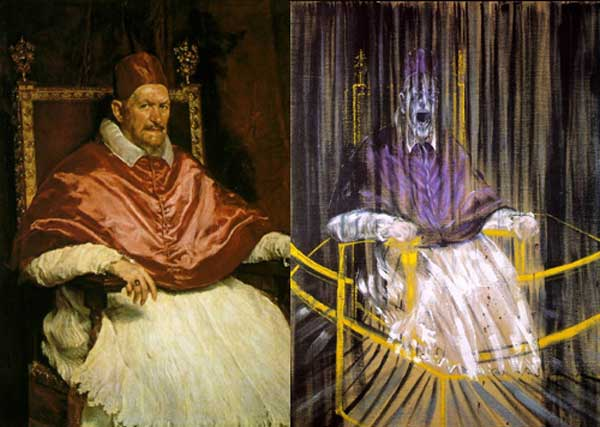
\includegraphics[height=5em]{bruyn-pope} \\
    $\mathbb{F}_1$
  \end{minipage}\quad
  \begin{minipage}{0.42\textwidth}
    \centering\small
    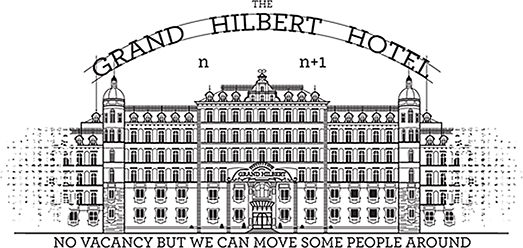
\includegraphics[height=5em]{hilbert-hotel} \\
    $\infty$
  \end{minipage}}
\end{frame}

{\usebackgroundtemplate{\begin{minipage}{\paperwidth}\vspace*{5.95cm}
\includegraphics[width=\paperwidth]{fr1}\end{minipage}}
\begin{frame}{The generic prime filter}
  \begin{wrapfigure}{r}{0.18\textwidth}
    \vspace*{-1.5em}
    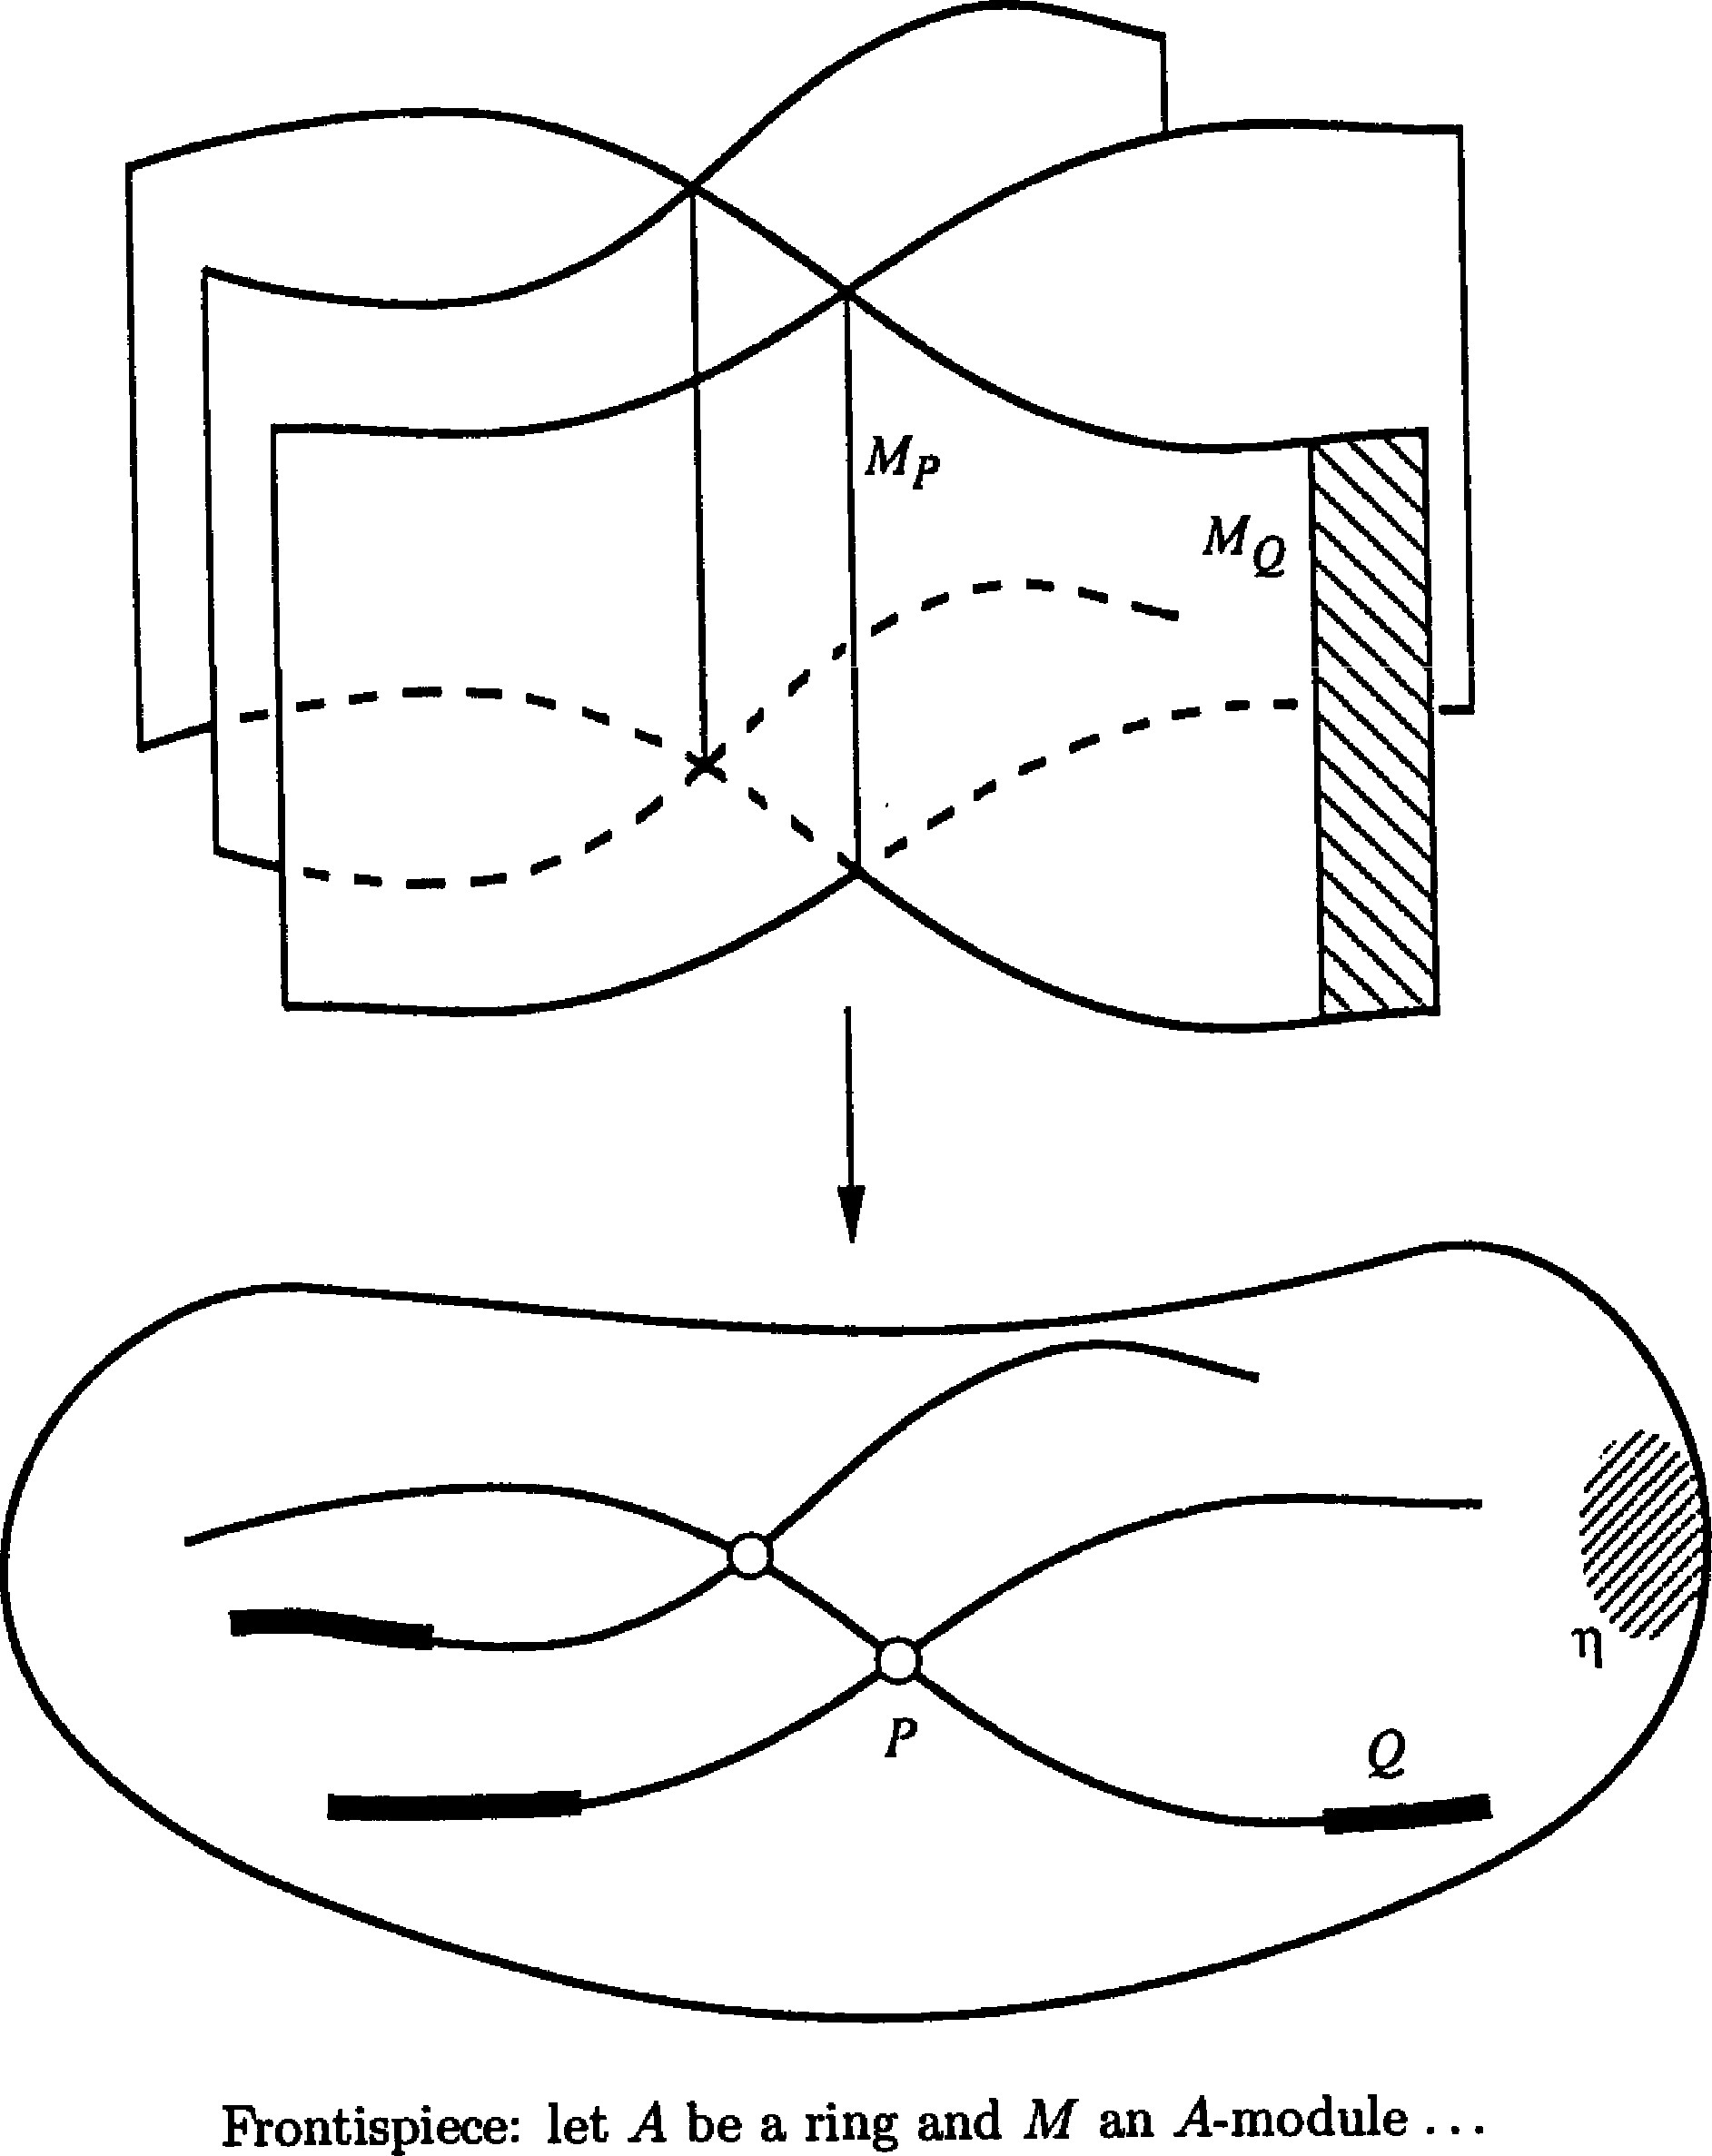
\includegraphics[width=0.20\textwidth]{miles-reid-frontispiece}
    \vspace*{-1.5em}
    \vspace*{-1.5em}
  \end{wrapfigure}

  \justifying
  Let~$A$ be a commutative ring with unit.
  Let~$M$ be an $A$-module. For any prime filter~$\ppp \subseteq A$, let
  \[ M_\ppp \defeq M[\ppp^{-1}] \defeq \{ \tfrac{x}{s} \,|\, x \in M, s \in \ppp \} \]
  be the \hil{stalk} of~$M$ at~$\ppp$.

  \visible<2->{\begin{varblock}{0.7\textwidth}{}
    The generic prime filter
    is a \hil{reification} of all prime filters into a single coherent
    entity.
  \end{varblock}}

  \only<3>{\textbf{Local-global principle.} \\\medskip
  {\small\centering\begin{tabular}{l@{$\quad\text{iff$^\star$}\quad$}l}
    % for all prime filters~$\ppp$, $A_\ppp$ is reduced & $A$ is reduced \\
    $M = 0$ & for all prime filters~$\ppp$, $M_\ppp = 0$. \\
    $M \to N$ is injective & for all prime filters~$\ppp$, $M_\ppp \to N_\ppp$ is injective. \\
    $M \to N$ is surjective & for all prime filters~$\ppp$, $M_\ppp \to N_\ppp$ is surjective. \\
    $f$ is nilpotent in~$A$ & for all prime filters~$\ppp$, $f \not\in \ppp$. \\
    ??? & for all prime filters~$\ppp$, $M_\ppp$ is fin.\@ generated over~$A_\ppp$. \\
    ???\!\!\!\!\!\!\!\!\phantom{$M$ is finite locally free} & for all prime filters~$\ppp$, $M_\ppp$ is finite free over~$A_\ppp$. \\
  \end{tabular}}}

  \only<4>{\textbf{Local-global principle.} Let~$\ppp_0$ be the \hil{generic prime filter}
  of~$A$. \\\medskip
  {\small\centering\begin{tabular}{l@{$\quad\text{iff}\quad$}l}
    % for all prime filters~$\ppp$, $A_\ppp$ is reduced & $A$ is reduced \\
    $M = 0$ & $M_{\ppp_0} = 0$. \\
    $M \to N$ is injective & $M_{\ppp_0} \to N_{\ppp_0}$ is injective. \\
    $M \to N$ is surjective & $M_{\ppp_0} \to N_{\ppp_0}$ is surjective. \\
    $f$ is nilpotent in~$A$ & $f \not\in \ppp_0$. \\
    $M$ is fin.\@ generated & $M_{\ppp_0}$ is fin.\@ generated. \\
    $M$ is finite locally free & $M_{\ppp_0}$ is finite free.
  \end{tabular}}}
\end{frame}}

\begin{frame}{The universal localization}
  Let~$A$ be a ring.

  The stalks~$A_\ppp$ are \hil{local rings}: If a finite sum of elements is
  invertible, then so is one of the summands.

  Is there a \hil{universal localization} of~$A$?
  \pause
  \[
    \xymatrix{
      A \ar[rd] \ar[rrr]^f &&& {\substack{\phantom{\text{local}}\\\text{\normalsize$R$}\\\text{local}}} \\
      & {\substack{\text{\normalsize$A'$}\\\text{local}}} \ar@{-->}_[@!35]{\text{local}}[rru]
    }
  \]
  \pause

  \justifying
  For a fixed local ring~$R$, the localization $A' \defeq A_\ppp$
  where~$\ppp \defeq f^{-1}[R^\times]$ would do the job.
  \pause

  \textbf{Fact.} A universal localization exists iff~$A$ has exactly one prime
  filter.
  \pause

  \textbf{Dream.} If only there was a \hil{generic prime filter}~$\ppp_0$,
  the universal localization would always exist and be given by~$A^\sim \defeq A_{\ppp_0}$!
\end{frame}

%{\usebackgroundtemplate{\begin{minipage}{\paperwidth}\vspace*{5.95cm}
\includegraphics[width=\paperwidth]{fr1}\end{minipage}}
%\begin{frame}{The generic prime filter}
%  \mbox{For~$A$-modules~$M$, let~$M^\sim \defeq M_{\ppp_0}$ be
%  the stalk at the generic prime filter.}
%
%  {\centering\begin{tabular}{l@{$\quad\Longleftrightarrow\quad$}l}
%    $x \not\in \ppp_0$ & $x$ is nilpotent \\
%    $x \in \ppp_0 \Rightarrow y \in \ppp_0$ & $x \in \sqrt{(y)}$ \\
%    % $x$ is regular in~$A^\sim$ & $x$ is regular in~$A$ \\
%    $A^\sim$ is reduced & $A$ is reduced \\
%    $A^\sim$ is an integral domain & $A$ is an integral domain \\
%    $M^\sim = 0$ & $M = 0$ \\
%    $M^\sim$ is fin.\@ generated over $A^\sim$ & $M$ is fin.\@ generated over~$A$ \\
%    $M^\sim$ is finite free & $M$ is finite locally free \\
%    % $M^\sim$ is flat over~$A^\sim$ & $M$ is flat over~$A$ \\
%    $M^\sim \to N^\sim$ is injective & $M \to N$ is injective \\
%    $M^\sim \to N^\sim$ is surjective & $M \to N$ is surjective
%  \end{tabular}}
%  \bigskip
%  \pause
% 
%  \subhead{$\boldsymbol{A^\sim}$ is better than~$\boldsymbol{A}$}
%  {\small\centering(Assume~$A$ reduced.)\par}
%  \begin{enumerate}[a]
%    \item $A^\sim$ is a \hil{field}: $\forall x\?A^\sim\_ (\neg(\exists y\?A^\sim\_
%      xy = 1) \Rightarrow x = 0)$.
%
%    %\item $A^\sim$ has \hil{$\boldsymbol{\neg\neg}$-stable equality}:
%    %  $\forall x,y\?A^\sim\_ \neg\neg(x = y) \Rightarrow x = y$.
%
%    \item \mbox{$A^\sim$ is \hil{anonymously Noetherian}.}\\[-1.2em]
%  \end{enumerate}
%\end{frame}}

{\usebackgroundtemplate{\begin{minipage}{\paperwidth}\vspace*{4.95cm}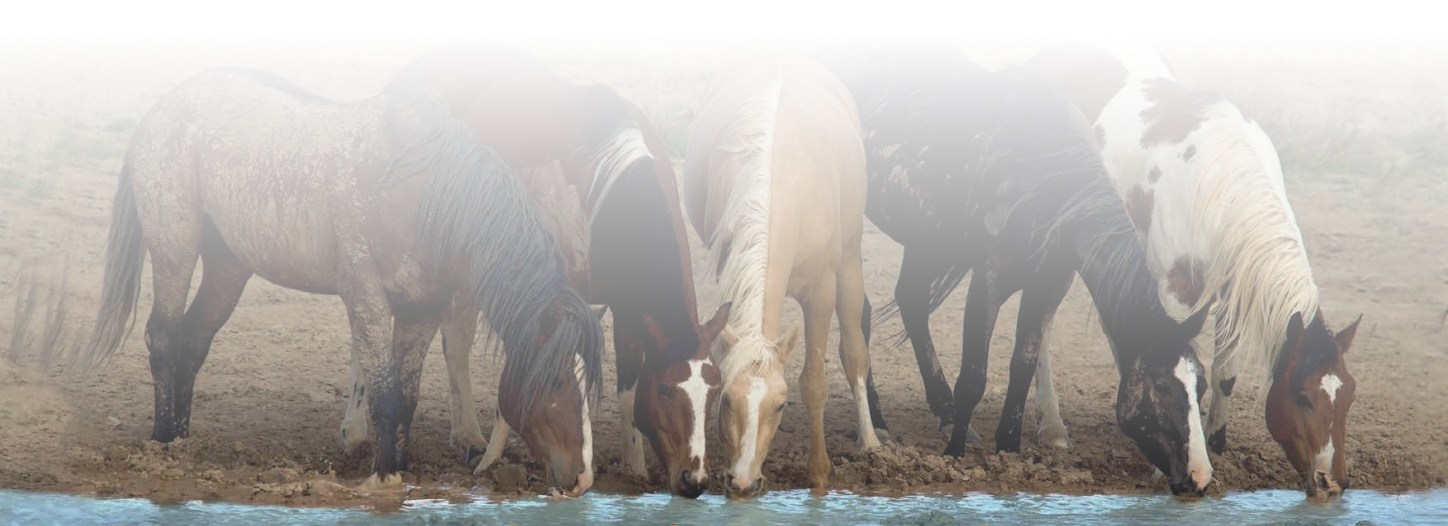
\includegraphics[width=\paperwidth]{topos-horses}\end{minipage}}
\begin{frame}{Generic models}
  \textbf{Theorem.} There is a \hil{generic ring}, a particular ring$^\star$
  such that for every$^{\star\star}$
  ring-theoretic statement~$\varphi$, the following are equivalent:
  \begin{enumerate}
    \item $\varphi$ holds for the generic ring.
    \item $\varphi$ holds for every ring.
    \item $\varphi$ is provable from the ring axioms.
  \end{enumerate}


  Similarly for every$^{\star\star\star}$ other theory in place of the theory of rings:
  \begin{itemize}
    \item[] \ldots{} the generic group, field, vector space, \ldots

    %-- \emph{the generic ring is neither~$\ZZ$ nor~$\ZZ[X]$}
    \item[] \ldots{} the generic prime ideal of a given ring~$A$ \ldots

    %-- \emph{don't confuse with the zero ideal}
    \item[] \ldots{} the generic surjection~$\NN \to X$ to a given set~$X$ \ldots

    %-- \emph{particularly useful in case~$X$ is not countable}
  \end{itemize}
  \bigskip
  \setlength\fboxsep{7pt}
  \visible<2->{\begin{minipage}{0.57\textwidth}
    \centering
    \colorbox{red!50}{Is~$1 + 1 = 0$ in the generic ring?} \\
    \scriptsize\color{white} \phantom{y}nonclassical truth values\phantom{y}
  \end{minipage}}
  \visible<3->{\begin{minipage}{0.42\textwidth}
    \centering
    \colorbox{mypurple!50}{The generic ring is a field.}
    \scriptsize\color{white} mysterious nongeometric sequents
  \end{minipage}}
  \bigskip
\end{frame}}

\begin{frame}[fragile]{Mathematical universes}
%  \begin{itemize}
%    \item The \hil{standard universe}~$V$
%    \item Gödel's \hil{constructible universe}~$L$
%    \item The \hil{ef{}fective topos}~$\Eff$
%    \item The topos~$\Sh(X)$ of set-valued \hil{sheaves} on a space~$X$
%    \item The \hil{classifying topos}~$\Set[\TT]$ of a geometric theory~$\TT$
%  \end{itemize}

  \tikzstyle{topos} = [draw=mypurple, very thick, rectangle, rounded corners, inner sep=5pt, inner ysep=10pt]
  \tikzstyle{title} = [fill=mypurple, text=white]

  % Taken from Todd Lehman (CC-BY-SA) at https://tex.stackexchange.com/a/44920/32372

\newcommand{\setisprime}[1]{
  % Sets \isprime based on #1.
  \ifnum#1=1 \gdef\isprime{0} \else \gdef\isprime{1} \fi
  \foreach \sip in {2, 3,5,...,#1} {
    \pgfmathparse{\sip*\sip>#1? 1:0}
    \ifthenelse{\pgfmathresult=1}{
      % Early-out if \sip^2 > #1.
      \breakforeach
    }{
      % Otherwise test if \sip divides #1.
      \pgfmathparse{Mod(#1,\sip)==0? 1:0}
      \ifthenelse{\pgfmathresult=1}{
        \gdef\isprime{0}
        \breakforeach
      }{}
    }
  }
}

\newcommand{\setxy}[1]{
  % Sets \x and \y to loction of cell #1.
  \pgfmathtruncatemacro{\x}{Mod(#1-1,\cols)}
  \pgfmathtruncatemacro{\y}{(#1-1) / \cols}
  \pgfmathtruncatemacro{\y}{\cols - 1 - \y}
  \pgfmathparse{2.5*(\x+.5)}\let\x\pgfmathresult
  \pgfmathparse{2.5*(\y+.5)}\let\y\pgfmathresult
}

\newcommand{\numlabel}[2]{
  % Draws label #2 at cell #1.
  \setxy{\n}
  \node[fill=none, text=black] at (\x,\y) {#2};
}

\newcommand{\drawpolygon}[2]{
  % Draws polygon with #2 vertexes at cell #1.
  \setxy{#1}
  \ifthenelse{#2>1}{ % Polygon must have at least 2 sides.
    \ifthenelse{#2<30}{ % Draw polygon if it has a small number of sides.
      \filldraw (\x,\y) +(90:1)
      \foreach \drawi in {1,...,#2} {-- +(\drawi/#2*360+90:1)} -- cycle;
    }{ % Else approximate with circle.
      \filldraw (\x,\y) circle(1);
    }
  }{}
}

\newcommand{\setpolygoncolor}[1]{
  % Sets color based on #1.
  \gdef\polycolor{black}
  \ifnum#1=2\gdef\polycolor{black!50!white}\fi
  \ifnum#1=3\gdef\polycolor{yellow!95!red}\fi
  \ifnum#1=5\gdef\polycolor{yellow!0!red}\fi
  \ifnum#1=7\gdef\polycolor{blue!75!green}\fi
  \ifnum#1=11\gdef\polycolor{blue!70!red}\fi
  \ifnum#1=13\gdef\polycolor{blue!40!red}\fi
  \ifnum#1=17\gdef\polycolor{green!50!blue}\fi
  \ifnum#1=19\gdef\polycolor{green!80!black}\fi
  \ifnum#1=23\gdef\polycolor{green!50!red}\fi
  \ifnum#1=29\gdef\polycolor{yellow!50!black}\fi
  \ifnum#1=31\gdef\polycolor{orange!50!black}\fi
  \ifnum#1=37\gdef\polycolor{red!50!black}\fi
  \ifnum#1=41\gdef\polycolor{purple!50!black}\fi
  \ifnum#1=43\gdef\polycolor{blue!50!black}\fi
  \ifnum#1=47\gdef\polycolor{green!50!black}\fi
  \ifnum#1=53\gdef\polycolor{white!50!black}\fi
  \ifnum#1=59\gdef\polycolor{white!50!black}\fi
  \ifnum#1=61\gdef\polycolor{white!50!black}\fi
  \ifnum#1=67\gdef\polycolor{white!50!black}\fi
}

\newcommand{\sieve}[2]{
  \def\cols{#1}
  \def\rows{#2}
  \begin{tikzpicture}[scale=.5]
  \pgfmathtruncatemacro{\nmax}{\rows * \cols}

  \foreach \n in {1,...,\nmax} {
    \begin{scope}[fill=gray, fill opacity=.05,
                  draw=gray, draw opacity=.10,
                  line width=4]
      \drawpolygon{\n}{\n}
    \end{scope}
    \setisprime{\n}
    \ifthenelse{\isprime=1}{
      \numlabel{\n}{\bf\n}
    }{
      \def\startintensity{.33}
      \def\incrintensity{.10}
      \def\intensity{\startintensity}

      \def\m{\n}
      \pgfmathtruncatemacro{\i}{\m / 2}

      % Divide \m by \i until \m is extinguished.
      % Increment \i each time it does not divide into \m.
      \whiledo{\m>1}{
        \setisprime{\i}
        \pgfmathparse{Mod(\m,\i)==0? 1:0}
        \ifthenelse{\pgfmathresult=1\and\isprime=1}{
          \setpolygoncolor{\i}
          \begin{scope}[fill=\polycolor, fill opacity=\intensity,
                        draw=\polycolor!85!black, draw opacity=\intensity,
                        line width=\intensity*1.5]
            \drawpolygon{\n}{\i}
          \end{scope}
          \pgfmathtruncatemacro{\m}{\m / \i}
          \pgfmathparse{\intensity + \incrintensity}\let\intensity\pgfmathresult
        }{
          \pgfmathtruncatemacro{\i}{\i - 1}
          \def\intensity{\startintensity}
        }
      }
      \begin{scope}[text=black, text opacity=.5]
        \numlabel{\n}{\scriptsize\n}
      \end{scope}
    }
  }

  \end{tikzpicture}
}


  \newcommand{\drawbox}[4]{
    \node[topos, #4] [fit = #3] (#1) {};
    \node[title] at (#1.north) {#2};
  }

  \newcommand{\muchstuff}{
    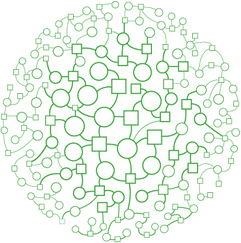
\includegraphics[height=3em]{filmat}
    \scalebox{0.5}{\sieve{14}{2}}
  }

  \newcommand{\muchstuffplaceholder}{
    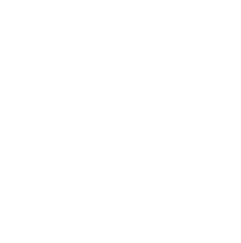
\includegraphics[height=3em]{filmat-placeholder}
    \scalebox{0.5}{\fakesieve{14}{2}}
  }

  \newcommand{\fewstuff}{
    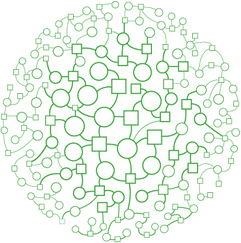
\includegraphics[height=3em]{filmat}
    \scalebox{0.5}{\sieve{7}{2}}
  }

  {\centering
  \begin{tikzpicture}
    \node[scale=0.4] (objs-set1) at (-4.0,-2.5) {
      \fewstuff
    };
    \node[scale=0.4] (objs-eff1) at (4.0,-2.5) {
      \fewstuff
    };
    \node[scale=0.4] (objs-sh1)  at (0,-2.5) {
      \fewstuff
    };

    \node (prop-set1) [below of=objs-set1, align=left] {
      The usual laws \\
      of logic hold.
    };

    \node (prop-eff1) [below of=objs-eff1, align=left] {
      Every function \\
      is computable.
    };

    \node (prop-sh1) [below of=objs-sh1, align=left] {
      The axiom of \\
      choice fails.
    };

    \drawbox{set1}{$\mathrm{Set}$}{(objs-set1) (prop-set1)}{}
    \drawbox{eff1}{Ef{}f}{(objs-eff1) (prop-eff1)}{tape}
    \drawbox{sh1}{$\mathrm{Sh}(X)$}{(objs-sh1) (prop-sh1)}{draw=none}
    \def\R{8pt}
    \begin{pgfonlayer}{background}
      \draw[decoration={bumps,segment length=8pt}, decorate, very thick, draw=mypurple]
        ($(sh1.south west) + (\R, 0)$) arc(270:180:\R) --
        ($(sh1.north west) + (0, -\R)$) arc(180:90:\R) --
        ($(sh1.north east) + (-\R, 0)$) arc(90:0:\R) --
        ($(sh1.south east) + (0, \R)$) arc(0:-90:\R) --
        cycle;
    \end{pgfonlayer}
  \end{tikzpicture}
  \par}

  \begin{itemize}
    \item For any topos~$\E$ and any statement~$\varphi$, we define the meaning of
    ``$\E \models \varphi$'' (``$\varphi$ holds in the internal universe
    of~$\E$'') using the \hil{Kripke--Joyal semantics}.
    \bigskip
    \item Any topos supports \hil{mathematical reasoning}:
    \medskip

    If~$\ \E \models \varphi\ $ and if~$\ \varphi$ entails~$\psi$
    \pointthis{<2>}{intuitionistically}{%
      no $\varphi \vee \neg\varphi$,\ \
      no $\neg\neg\varphi \Rightarrow \varphi$,\ \
      no axiom of choice},
    then~$\ \E \models \psi$.
  \end{itemize}
\end{frame}

\newcommand{\expl}[2]{
  ``$\Eff \models \!\!\text{\normalnumber{#1}}$\!'' means: #2
}

\begin{frame}{Exploring the \effective topos}
  \vspace*{-1em}
  \begin{center}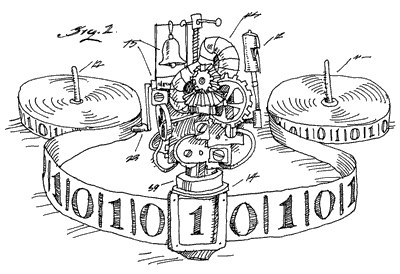
\includegraphics[width=0.4\textwidth]{turing-machine}\end{center}
  \small
  \begin{tabular}{@{\!\!\!\!\!\!\!\!}l@{\,}lll}
    \toprule
    & Statement & in $\Set$ & in $\Eff$ \\
    \midrule
    \normalnumber{1} & Every natural number is prime or not prime. & \cmark{} (trivially) & \cmark \\
    \normalnumber{2} & There are infinitely many primes. & \cmark & \cmark \\
    \normalnumber{3} & Every map $\NN \to \NN$ is constantly zero or not. & \cmark{} (trivially) & \xmark \\
    \normalnumber{4} & Every map $\NN \to \NN$ is computable. & \xmark & \cmark{} (trivially) \\
    \normalnumber{5} & Every map $\RR \to \RR$ is continuous. & \xmark & \cmark \\
    %\normalnumber{6} & Markov's principle holds. & \cmark{} (trivially) & \cmark \\
    %\normalnumber{7} & Heyting arithmetic is categorical. & \xmark & \cmark \\
    \bottomrule
  \end{tabular}
  \medskip

  \only<2>{\expl{1}{There is a machine which determines of any given
  number whether it is prime or not.}}
  \only<3>{\expl{2}{There is a machine producing arbitrarily many
  primes.}}
  \only<4>{\expl{3}{There is a machine which, given a machine
  computing a map~$f : \NN \to \NN$, determines whether~$f$ is constantly
  zero or not.}}
  \only<5>{\expl{4}{There is a machine which, given a machine
  computing a map~$f : \NN \to \NN$, outputs a machine
  computing~$f$.}}
\end{frame}

\begin{frame}{The classifying topos as a local lens}
  \small
  \begin{itemize}
    \item\justifying For ring elements~$f \in A$ and formulas~$\varphi$, we
    define~\speak{D(f)}{\varphi} (``$\varphi$~holds on (and beyond)
    stage~$D(f)$'') by the following clauses.
    \item\justifying A formula~$\varphi$ holds in the classifying topos of the theory of
    prime filters of~$A$ iff~\speak{D(1)}{\varphi}.
  \end{itemize}

  \renewcommand{\arraystretch}{1.3}
  \begin{tabular}{p{0.31\textwidth}@{\ iff\ }p{0.75\textwidth}}
    \speak{D(f)}{\forall x\?A^\sim\_ \varphi(x)} &
      for all~$g \in A$ and~$x_0 \in A[g^{-1}]$, \speak{D(fg)}{\varphi(x_0)} \\
    \speak{D(f)}{\varphi \Rightarrow \psi} &
      for all~$g \in A$, \speak{D(fg)}{\varphi} implies~\speak{D(fg)}{\psi} \\
    \speak{D(f)}{\varphi \vee \psi} &
      there is a partition~$f^n = f g_1{+}\cdots{+}f g_m$ s.\@ th.\@
      \phantom{lollollololllol}
      \phantom{lol} for each~$i$,
      \speak{D(fg_i)}{\varphi}
      or \speak{D(fg_i)}{\psi} \\
    \speak{D(f)}{\bot} & $f$ is nilpotent \\
    \speak{D(f)}{x \in \ppp_0} & $f \in \sqrt{(x)}$
  \end{tabular}
  \bigskip
  \pause


  \textbf{Example.}\par
  \scriptsize
  \vspace*{-1.5em}
  \begin{align*}
    & \text{\speak{D(1)}{\text{`$x$ is not invertible'}}}
    \ \ \ \ \text{iff}\ \ \ \ \text{\speak{D(1)}{\text{`$x$ is invertible'} \Rightarrow \bot}} \\
    \text{iff}\ \ \ \ & \text{for all~$g \in A$, if \speak{D(g)}{\text{`$x$ is invertible'}} then~\speak{D(g)}{\bot}} \\
    \text{iff}\ \ \ \ & \text{for all~$g \in A$, if $x$ is invertible in~$A[g^{-1}]$
  then~$g$ is nilpotent}
    \ \ \ \ \text{iff}\ \ \ \ \text{$x$ is nilpotent}.
  \end{align*}
\end{frame}

\begin{frame}{Applications of the generic prime filter}
  \small
  \subhead{Injective matrices}
  \begin{varblock}{\textwidth}{Injective matrices}
    \justifying
    \textbf{Theorem.}
    Let~$M$ be an injective matrix with more columns than rows over a ring~$A$.
    Then~$1 = 0$ in~$A$.
  \end{varblock}
  \pause

  \justifying
  \textbf{Proof.} \bad{Assume not.} Then there is a \bad{minimal
  prime ideal} $\ppp \subseteq A$. The matrix is injective over the \bad{field}~$A_\ppp$;
  contradiction to basic linear algebra.\qed\medskip
  \pause

  \textbf{Proof.} \simplespeak{$M$ is also injective as a matrix over~$A^\sim = A_{\ppp_0}$.
  This is a contradiction by basic intuitionistic linear
  algebra.} Thus~\simplespeak{$\bot$}. Hence~$1 = 0$ in~$A$.\qed
  \bigskip
  \pause

  \subhead{Grothendieck's generic freeness}
  \begin{varblock}{\textwidth}{Generic freeness\phantom{p}}
    \justifying
    \textbf{Theorem.}
    Let~$M$ be a finitely generated~$A$-module.
    If~$f = 0$ is the only element of~$A$ such that~$M[f^{-1}]$ is a
    free~$A[f^{-1}]$-module, then~$1 = 0$ in~$A$.
  \end{varblock}

  \justifying
  \textbf{Proof.} The claim amounts to \simplespeak{$M^\sim$ is \hil{not not} free}.
  This statement follows from basic intuitionistic linear algebra over the
  field~$A^\sim$.\qed
\end{frame}

\end{document}

illustration:
phantoms

0 Mathematical phantoms
"One of the recurring themes of mathematics, and one that I have always found
seductive, is that of the nonexistent entity which ought to be there but
apparently is not; which nevertheless obtrudes its effects so convincingly that
one is forced to concede a broader notion of existence."  -- Gavin Wraith

animation of extensions of the natural number line?
